 %%%%%%%%%%%%%%%%%%%%%%%%%%%%%%%%%%%%%%%%%%%%%%%%%%%%

\documentclass[12pt]{article}
\usepackage{epsf}
\usepackage{amsmath}
\usepackage{amsfonts}
\usepackage{amssymb}
\usepackage{graphicx}
\usepackage{color}
\usepackage{psfrag}
\usepackage{cite}
\usepackage{rotating}
\usepackage{wrapfig,lipsum,booktabs}
\usepackage{lscape}
\usepackage{longtable}
\usepackage{hyperref}

% For use with xfig+(PS+Latex or PDF+Latex) export.
\usepackage{ifpdf}
\newcommand{\inputfig}[1]{
\ifpdf
  \input{#1.pdf_t}
  \else
  \input{#1.pstex_t}
\fi}


\renewcommand{\topfraction}{0.8}
\renewcommand{\bottomfraction}{0.8}
\renewcommand{\baselinestretch}{1.3}
% shortcuts
\newcommand{\bmat}{\left(\begin{array}}
\newcommand{\emat}{\end{array}\right)}
\def\NPB#1#2#3{Nucl. Phys. B{#1} (19#2) #3}
\def\PLB#1#2#3{Phys. Lett. B{#1} (19#2) #3}
\def\PLBold#1#2#3{Phys. Lett. {#1B} (19#2) #3}
\def\PRD#1#2#3{Phys. Rev. D{#1} (19#2) #3}
\def\PRL#1#2#3{Phys. Rev. Lett. {#1} (19#2) #3}
\def\PRT#1#2#3{Phys. Rep. {#1} C (19#2) #3}
\def\MODA#1#2#3{Mod. Phys. Lett.  {#1} (19#2) #3}
%\def\mb#1{\mbox{\boldmath $#1$}}
\def\Deq#1{\mbox{$D$=#1}}
\def\Neq#1{\mbox{$N$=#1}}
\def\preal{{\rm Re\,}}
\def\pim{{\rm Im\,}}
\def\ds{\displaystyle}
\def\yzero{\smash{\hbox{$y\kern-4pt\raise1pt\hbox{${}^\circ$}$}}}
\def\p{\partial}
\def\a{\alpha}
\def\b{\beta}
\def\g{\gamma}
\def\d{\delta}
\def\be{\begin{equation}}
\def\ee{\end{equation}}
\def\bea{\begin{eqnarray}}
\def\eea{\end{eqnarray}}
\def\beq{\begin{equation}}
\def\eeq{\end{equation}}
\def\beqa{\begin{eqnarray}}
\def\eeqa{\end{eqnarray}}
\def\Om{\Omega}
\def\om{\omega}
\def\th{\theta}
\def\vt{\vartheta}
\def\vphi{\varphi}
\def\-{\hphantom{-}}
\def\ov{\overline}
\def\s2{\frac{1}{\sqrt2}}
\def\wh{\widehat}
\def\wt{\widetilde}
\def\oh{\frac{1}{2}}
\def\beq{\begin{equation}}
\def\eeq{\end{equation}}
\def\beqa{\begin{eqnarray}}
\def\eeqa{\end{eqnarray}}
\def\tr{{\rm tr \,}}
\def\Tr{{\rm Tr \,}}
\def\Pf{{\rm Pf \,}}
\def\nn{\nonumber}
\def\diag{{\rm diag \,}}
\def\IF{\relax{\rm I\kern-.18em F}}
\def\II{\relax{\rm I\kern-.18em I}}
%\def\IP{\relax{\rm I\kern-.18em P}}
%\def\IC{\relax\hbox{\kern.25em$\inbar\kern-.3em{\rm C}$}}
%\def\IR{\relax{\rm I\kern-.18em R}}
\def\hm{\relax{n_H}}
\def\vac{|0 \rangle}
\def\vm{\relax{n_V}}
\def\ca{{\cal A}}
\def\cc{{\cal C}}
\def\ck{{\cal K}}
\def\ci{{\cal I}}
\def\cu{{\cal U}}   
\def\cg{{\cal G}}
\def\cn{{\cal N}}
\def\cl{{\cal L}}
\def\cam{{\cal M}}
\def\cp{{\cal P}}
\def\ct{{\cal T}}
\def\cv{{\cal V}}
\def\cz{{\cal Z}}
\def\ch{{\cal H}}
\def\cf{{\cal F}}
\def\tv{\tilde v}
\def\Dsl{\,\raise.15ex\hbox{/}\mkern-13.5mu D} %this one can be subscripted
%\def\IZ{Z\kern-.4em  Z}
\def\id{{\rm I}}
%\def\cp#1{\relax\ifmmode {\IP\kern-2pt{}_{#1}}\else $\IP\kern-2pt{}_{#1}$\fi}

\def\IC{{\bf C}}
\def\IS{{\bf S}}
\def\IR{{\bf R}}
\def\IZ{{\bf Z}}
\def\IX{{\IZ}}
\def\IT{{\bf T}}
\def\IP{\bf P}
\def\CL{{\cal L}}
\def\CM{{\cal M}}
\def\CN{{\cal N}}
\def\CO{{\cal O}}
\newcommand{\mf}[1]{{\marginpar{\footnotesize{ #1}}}}


%my defs
\def\k{\kappa}
\def\vt{\vartheta}
\def\vphi{\varphi}
\def\eps{\epsilon}

\def\im{{\rm Im}\,}   
\def\re{{\rm Re}\,}   

\def\A{{\bf A}}   
\def\B{{\bf B}}
\def\ent{{\bf Z}}
\def\C{{\bf C}}
\def\ti{\times}
\def\OR{\Omega {\cal R}}  
\def\R{{\cal R}}
\def\ca{{\cal A}}
\def\lam{\lambda}
\def\raw{\rightarrow}
\def\Raw{\Rightarrow}
\def\G{\Gamma}
\def\ep{\epsilon}
\def\arr{\arrowvert}
\def\Arr{\Arrowvert}

\newcommand{\drawsquare}[2]{\hbox{%
\rule{#2pt}{#1pt}\hskip-#2pt%  left vertical
\rule{#1pt}{#2pt}\hskip-#1pt%  lower horizontal
\rule[#1pt]{#1pt}{#2pt}}\rule[#1pt]{#2pt}{#2pt}\hskip-#2pt%  upper horizontal
\rule{#2pt}{#1pt}}% right vertical

\newcommand{\sbt}{\,\begin{picture}(-1,1)(-1,-3)\circle*{4}\end{picture}\ }

% Young tableaux
\newcommand{\fund}{\raisebox{-.5pt}{\drawsquare{6.5}{0.4}}}%  fund
\newcommand{\Ysymm}{\raisebox{-.5pt}{\drawsquare{6.5}{0.4}}\hskip-0.4pt%
        \raisebox{-.5pt}{\drawsquare{6.5}{0.4}}}%  symmetric second rank
\newcommand{\Yasymm}{\raisebox{-3.5pt}{\drawsquare{6.5}{0.4}}\hskip-6.9pt%
        \raisebox{3pt}{\drawsquare{6.5}{0.4}}}%  antisymmetric second rank
\newcommand{\antifund}{\overline{\fund}}
\newcommand{\bYasymm}{\overline{\Yasymm}}
\newcommand{\bYsymm}{\overline{\Ysymm}}

\setlength\fboxsep{3.0mm}


%%%%%%%%%%%%%%%%%%%%%%%%% rotate.sty
%
%   These macros allow you to rotate or flip a \TeX\ box.  Very useful for
%   sideways tables or upsidedown answers.
%
%   To use, create a box containing the information you want to rotate.
%   (An hbox or vbox will do.)  Now call \@rotr\boxnum to rotate the
%   material and create a new box with the appropriate (flipped) dimensions.
%   \@rotr rotates right, \@rotl rotates left, \@rotu turns upside down, and
%   \@rotf flips.  These boxes may contain other rotated boxes.
%
\catcode`\@=11   
\newdimen\@rotdimen
\newbox\@rotbox  

\def\@vspec#1{\special{ps:#1}}%  passes #1 verbatim to the output
\def\@rotstart#1{\@vspec{gsave currentpoint currentpoint translate
   #1 neg exch neg exch translate}}% #1 can be any origin-fixing transformation
\def\@rotfinish{\@vspec{currentpoint grestore moveto}}% gets back in synch 
%
%   First, the rotation right. The reference point of the rotated box
%   is the lower right corner of the original box.
%
\def\@rotr#1{\@rotdimen=\ht#1\advance\@rotdimen by\dp#1%
   \hbox to\@rotdimen{\hskip\ht#1\vbox to\wd#1{\@rotstart{90 rotate}%
   \box#1\vss}\hss}\@rotfinish}
%
%   Next, the rotation left. The reference point of the rotated box
%   is the upper left corner of the original box.
%
\def\@rotl#1{\@rotdimen=\ht#1\advance\@rotdimen by\dp#1%
   \hbox to\@rotdimen{\vbox to\wd#1{\vskip\wd#1\@rotstart{270 rotate}%
   \box#1\vss}\hss}\@rotfinish}%
%
%   Upside down is simple. The reference point of the rotated box
%   is the upper right corner of the original box. (The box's height
%   should be the current font's xheight, \fontdimen5\font,
%   if you want that xheight to be at the baseline after rotation.)
%
\def\@rotu#1{\@rotdimen=\ht#1\advance\@rotdimen by\dp#1%
   \hbox to\wd#1{\hskip\wd#1\vbox to\@rotdimen{\vskip\@rotdimen
   \@rotstart{-1 dup scale}\box#1\vss}\hss}\@rotfinish}%
%
%   And flipped end for end is pretty ysae too. We retain the baseline.   
%   
\def\@rotf#1{\hbox to\wd#1{\hskip\wd#1\@rotstart{-1 1 scale}%
   \box#1\hss}\@rotfinish}%
%   
%   Now the user interface for LaTeX:  \rotate[type]{text} where
%   ``type'' is `l' for left, `r' for right, `u' for upside-down, or
%   `f' for flip.  `l' is the default.
%
\def\rotate{\@ifnextchar[{\@rotate}{\@rotate[l]}}
\def\@rotate[#1]#2{\setbox\@rotbox=\hbox{#2}\@nameuse{@rot#1}\@rotbox}

\catcode`\@=12
%%%%%%%%%%%%%%%%%  End of rotate.sty

\topmargin
-1.5cm
\textwidth
15.5cm
\textheight
23.5cm
\oddsidemargin
0.7cm
\evensidemargin
1.2cm


\title{{\LARGE TARGet}}

\makeatletter
\def\@maketitle{
\begin{center}
\vspace*{5.5cm}{\Huge \bfseries \sffamily \@title }\\[4ex] 
{\Large User's Guide}\\[6ex]


\includegraphics[width = 60mm]{logo.png}\\[12ex]

\@date\\[6ex]

\end{center}}
\makeatother

\begin{document}
\maketitle

\newpage

\section{Introduction}
\label{sec1}

TARGet is a light-weight application for reconstructing non-vertical evolutionary histories from sampled genetic sequences. TARGet makes use of persistent homology \cite{ph, ph2}, a tool from topological data analysis, to infer information about the minimal set of reticulate events (recombination, re-assortment, etc) that are needed 
to explain a sequence alignment, under the assumption of no convergent evolution. It exploits a sequence partitioning strategy similar to that of ref.~\cite{mg}, but the topological nature of TARGet permits inferring phylogenetic information about reticulate events, like the participating gametes or the associated genetic scales. Specifically, TARGet computes the extended first-homology barcode of the sequence alignment and attempts to reconstruct the topological ancestral recombination graph (tARG), which is closely related (in most cases actually identical) to minimal ARGs \cite{target}. 

The advantage of working with barcodes and tARGs is that they can be computed in polynomial time, without having to perform exhaustive explorations of the ARG space. Hence, as opposed to standard methods of ancestral recombination graph (ARG) reconstruction, TARGet is a fast multi-threaded algorithm that can be applied to large datasets, consisting of hundreds of genetic sequences. It is therefore a great tool for exploring reticulate evolution not only in virus and bacteria, but also in eukaryotes.

TARGet is distributed under the GNU General Public License (GPL v3). It is fully written in Python 2.7, but heavily relies on \href{http://www.mrzv.org/software/dionysus/}{Dionysus} C++ library for persistent homology computations. It runs in Windows, Mac OS and Unix systems, provided all dependences are installed. If you use TARGet for your research, please include \cite{target} in your references. 

\subsection*{Installation}

To run TARGet, the following free software is required in the system:
\begin{itemize}
\item[-] \href{https://www.python.org/}{Python 2.7.} (Python 3 is currently not supported.)
\item[-] \href{http://www.cmake.org/}{CMake.}
\item[-] \href{http://www.boost.org/}{Boost C++ libraries,} including Boost.Python.
\item[-] \href{https://networkx.github.io/}{NetworkX} package for Python.
\end{itemize}

\noindent For optimal visualization results it is also recommended to have \href{http://www.graphviz.org/}{Graphviz} tools and \href{http://pygraphviz.github.io/}{PyGraphviz} installed, although they are not strictly required.

Once the above dependences are installed in the system, you can unpack and build TARGet by typing the following commands in a terminal:

\texttt{tar -xvzf TARGet.tar.gz}

\texttt{cd TARGet}

\texttt{mkdir build}

\texttt{cd build}

\texttt{cmake ..}

\texttt{make}

The Python executable is in directory \texttt{TARGet}. You can check that TARGet has been correctly installed by running it on the test or on the example FASTA files that come with the distribution:

\texttt{./TARGet test.fa}

\noindent or

\texttt{python TARGet test.fa}


\subsection*{Troubleshooting}

These are some potential problems that can happen during the installation procedure, and their solution:

\begin{itemize}
\item[-] On Mac OSX, CMake often has issues finding the correct python path. 
If that is the case, uncomment the following three lines in file 
CMakeLists.txt, replacing the directories for the appropriate ones 
in your system,

\texttt{set (PYTHON\_EXECUTABLE /usr/local/bin/python2.6)}

\texttt{set (PYTHON\_INCLUDE\_DIR /usr/local/include/python2.6)}

\texttt{set (PYTHON\_PATH /usr/local/lib/libpython2.6.dylib)}

and run \texttt{cmake} and \texttt{make} again.

\item[-] Some compiler versions may raise the following error:

\texttt{error: unrecognized command line option "-ftemplate-depth=256"}

If that is the case, replace the following line in CMakeList.txt,

\texttt{add\_definitions  \qquad \qquad              (-ftemplate-depth=256)}

by,

\texttt{add\_definitions   \qquad \qquad          (-ftemplate-depth-256)}

and run cmake and make again.

\item[-] It is important to run TARGet using the same version of Python that 
was used to compile TARGet and Boost libraries.

\end{itemize}

\section{Running TARGet}

\subsection*{Input file}

The standard TARGet input is a FASTA file containing a DNA sequence alignment. For better performance, it is recommended to remove duplicated sequences from the input file before running TARGet. The current version cannot deal properly with large gaps (more than 2 or 3 bases long), so it is also advised to remove those loci from the alignment. A suitable gap treatment will be implemented in next versions of TARGet.

Alternatively, the input file can contain only segregating sites (in bi-allelic 0/1 format). For instance:

\texttt{>Sequence ID 1}

\texttt{11110000}

\texttt{>Sequence ID 2}

\texttt{00001100}

\texttt{\ldots}

\noindent Note, however, that all positions in TARGet's output will refer in that case to segregating sites and not to genomic positions.

\subsection*{Command line options}

TARGet can be run with default parameters by just typing:

\texttt{./TARGet <input file>}

\noindent or

\texttt{python TARGet <input file>}

\noindent where \texttt{<input file>} is the name of the FASTA file containing the alignment. However, there are several command line options that may result useful:

\subsubsection*{\texttt{-c \#}}

TARGet is a multi-threaded algorithm. By default it will run in a single CPU core, but you can specify a higher number of cores with the command line option \texttt{-c \#}, where \texttt{\#} is the number of cores that TARGet can use.

\subsubsection*{\texttt{-o <prefix>}}

TARGet produces four output files. By default these are named:

\texttt{out.b1.txt}

\texttt{out.bars.txt} 

\texttt{out.targ}

\texttt{out.gexf}

\noindent A different prefix (instead of \texttt{out}) for the output files can be specified with the command line option \texttt{-o <prefix>}.

\subsubsection*{\texttt{-s \#}, \texttt{-t \#} and \texttt{-w \#}}

As already stated, TARGet makes use of a sequence partitioning strategy similar to that of Myers and Griffiths~\cite{mg}. In most cases, considering all possible sequence partitions is  unnecessary and computationally too expensive. The number of sequence partitions that TARGet computes can be limited by the maximum and minimum numbers of segregating sites within each segment, and by the maximum distance (measured in number of segregating sites) between segment extrema. The default values for these three quantities are 2, 5 and 13, respectively. The user can specify different values by means of the command line options \texttt{-s \#}, \texttt{-t \#} and \texttt{-w \#}, respectively, where \texttt{\#} indicates the number of segregating sites.

In general, taking large values for \texttt{-s \#} and \texttt{-w \#} can increase substantially the running time and memory requirements. We find that a useful strategy is to first run TARGet with default parameters. Then, increase as much as possible the number of segregating sites within segments using \texttt{-s \#}. This will improve the sensitivity and the genetic scale range. If the value of \texttt{-s \#} approaches that of \texttt{-w \#}, and running time and memory requirements are still good, you may want to also increase the maximum distance between segment extrema using \texttt{-w \#}. Sometimes you may capture large scale recombination loops, even if they could be split in smaller ones. Increasing \texttt{-t \#} is a good strategy in those situations.

\subsubsection*{\texttt{-e}}

It excludes from the computation segregating sites that are compatible with all the other sites in the sequence alignment. This speeds up the computation, but can slightly alter the genetic scales of some of the bars in the extended first-homology barcode.

\subsubsection*{\texttt{-n}}

By default, when TARGet finishes computing the extended barcode and tARG of the sequence alignment, it opens a graphical interface that allows exploring the results interactively. The use of the graphical interface is described below. The user may want to change this behavior, so that the graphical interface is not automatically opened. This can be achieved by means of the command line option \texttt{-n}. Note that it is always possible to resume previous results by using the command line option \texttt{-l}, described below, without having to recompute the tARG.

\subsubsection*{\texttt{-l}}

One of the three output files that TARGet produces is a binary file (by default named \texttt{out.targ}) containing all the information required to open a previously computed extended barcode and tARG in the graphical interface. You may use the command line option \texttt{-l} to open a \texttt{.targ} file. In this case the input file is not a FASTA file, but a \texttt{.targ} file.

\section{Understanding the output}

TARGet produces an extended barcode associated to the sequence alignment and attempts to reconstruct the tARG. Each bar in the extended barcode represents a reticulate event in the sample history. Bar positions and lengths are related to the genetic scales of the gametes that took part in the reticulate event, measured in number of mutations. Assuming good sampling density, reticulate events involving genetically very different parental sequences (e.g. recombination of strains that diverged long time ago) are represented by long bars at high genetic scales in the barcode, whereas reticulate events involving closely related parental sequences appear as short bars at low genetic scales.

For the sake of illustration, consider a sample of 7 sequences with the following genotype (these can be found in the file \texttt{test.fa}):

0\ : \ \texttt{1 1 1 1 0 0 0 0}

1\ : \ \texttt{0 0 0 0 1 1 0 0}

2\ : \ \texttt{0 0 0 0 1 1 0 1}

3\ : \ \texttt{1 1 1 1 1 1 1 0}

4\ : \ \texttt{1 1 1 1 0 0 1 0}

5\ : \ \texttt{0 0 0 0 0 0 0 0}

6\ : \ \texttt{1 1 1 1 1 1 0 0}

\noindent Minimal histories of the sample involve 2 recombination events under the assumption of no convergent evolution. An example of minimal history is shown in figure \ref{fig1}a. The corresponding tARG, depicted in figure \ref{fig1}b, represents the unrooted topology of minimal ARGs \cite{target}. Hence, it contains the two loops present in the minimal ARG of figure \ref{fig1}a, and allows identifying the specific gametes that participate in each recombination event. 

The extended barcode of the sample is shown in figure \ref{fig1}c. It has two bars, corresponding to the two recombination events of minimal ARGs. The shortest bar is associated to the recombination between gametes 0 and 3, which differ on a single nucleotide. The longest bar is associated to the recombination between gametes 0 and 1, which differ in 6 nucleotides. The location of recombination break points is also shown in figure \ref{fig1}c.

\begin{figure}[!ht]
\centering
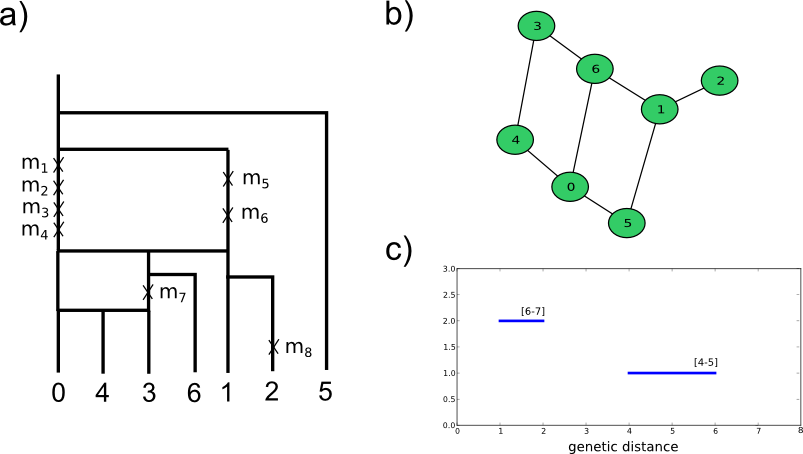
\includegraphics[width=15.8cm, angle=0]{draw.png}
\caption{a) Example of minimal ARG describing a minimal evolutionary history for the sample of 7 sequences considered in the text. Mutation events in the $i$-th position are represented as $m_i$. Root node is marked in red and leaf nodes are marked in green. The ARG involves two recombination events. b) tARG associated to the sample. c) Extended barcode associated to the sample.
\label{fig1}}
\end{figure} 

\noindent These results can be simply obtained by running

\texttt{./TARGet -s 8 test.fa}

\noindent Barcodes are relatively stable against sampling. For instance, in the above example we would obtain the same barcode if we remove sequences 0, 2 and 6 from the sample. 

\subsection*{Graphical interface}

TARGet has a interactive graphical interface that permits exploring the results. A snapshot of the interface is shown in figure \ref{fig2}. The interface consists of 5 different panels. Panel 1 contains the extended barcode of the sequence alignment, depicting genetic scales of reticulate events, as described above. Panel 2 contains the reconstructed tARG of the sample. Panel 5 represents a set of intervals on the genetic sequence, indicating the number of reticulate events of the tARG (the so-called \emph{first Betti number}) with break points in the interval. In addition, loci at which the Hudson-Kaplan's four gamete test \cite{hk} fails across consecutive segregating sites are also indicated in panel 5 (red lines). Positions in that panel refer to genomic positions, except when the input file contains only segregating sites. 

When selecting a bar in panel 1, the corresponding loop is marked red in the tARG representation of panel 2, and panel 3 list the identifiers of the genetic sequences that participate in that reticulate event (see figure \ref{fig2}). 

Generally, the extended barcode is built out of various sequence blocks \cite{target}, following a partitioning algorithm similar to that of \cite{mg}. Hence, when selecting a bar in panel 1, other bars belonging to the same building block are also highlighted in yellow, as well as the corresponding cycles in panel 2. In addition, panel 4 indicates the part of the genetic sequence that is associated to that building block.

\begin{figure}[!ht]
\centering
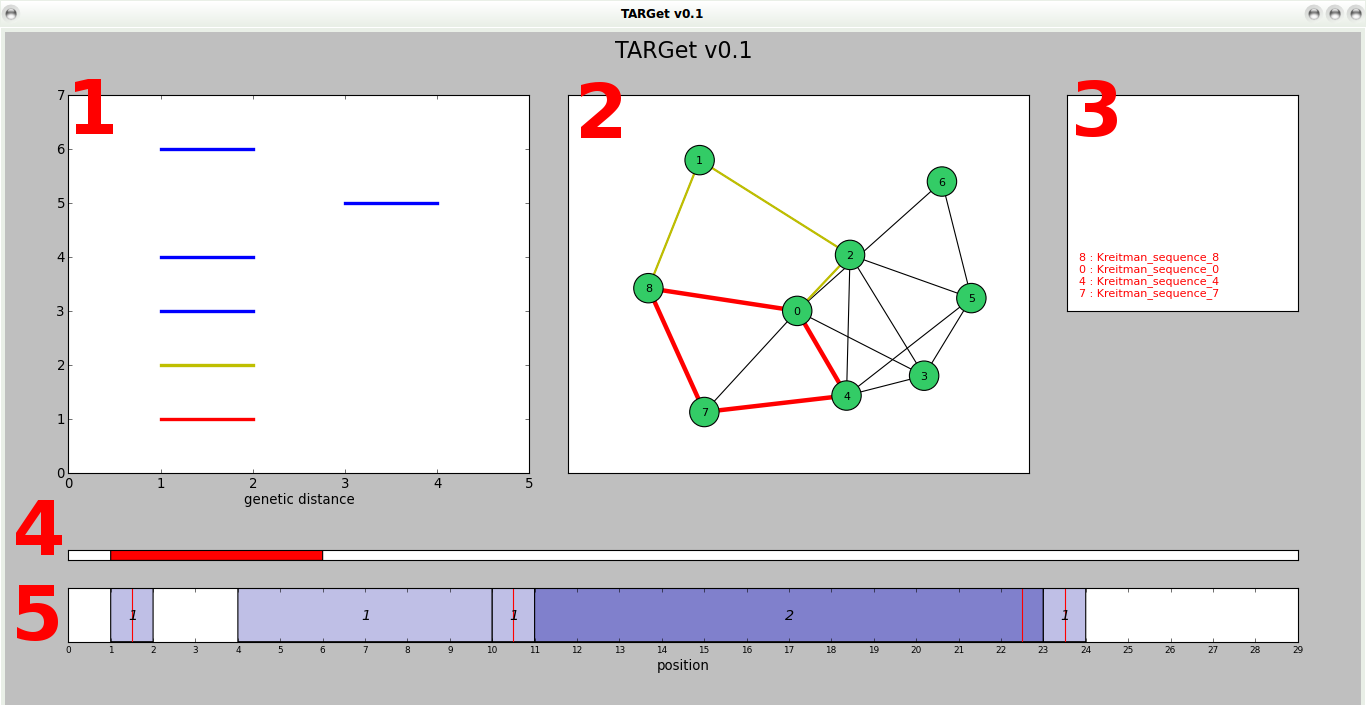
\includegraphics[width=15.cm, angle=0]{Screenshot.png}
\caption{Graphical interface of TARGet.
\label{fig2}}
\end{figure} 


\subsection*{Output files}

TARGet produces four output files, by default named \texttt{out.bars.txt}, \texttt{out.b1.txt}, \texttt{out.targ} and \texttt{out.gexf}. We have described above the use of the binary file \texttt{out.targ}, containing all the information required to resume a graphical session.

The file \texttt{out.bars.txt} contains a tab separated table listing all reticulate events in the extended barcode. The format is:

\texttt{birth\ \ \ \ \ death\ \ \ \ \ generators\ \ \ \ \ start\ \ \ \ \ end}

\noindent Each row represents a single reticulate event in the tARG. The first two columns in the table contain the genetic scales of the two bar extrema in the extended barcode. The third column contains a list of the edges that make the corresponding loop in the tARG. Each edge is given by a pair of sequences, where sequences are denoted by integers starting from 0 in the same order as they appear in the input file. The last two columns contain respectively the start and end positions of the genomic segment associated to the building block containing the reticulate event \cite{target}. 

The file \texttt{out.b1.txt} contains a tab separated table with columns:

\texttt{start\ \ \ \ \ end\ \ \ \ \ b1}

\noindent Each row represents an interval of the genetic sequence constraining as much as possible the location of reticulate events break points. The first and second columns of the table contain the start and end positions of the interval, respectively. The third column is the number of reticulate events with break points in that interval. Note that currently the algorithm that TARGet uses to constrain the location of break points is sub-optimal, and in complex situations some of the reticulate events listed in the file \texttt{out.bars.txt} may be missing in the file \texttt{out.b1.txt}.

All positions listed in the columns \texttt{start} and \texttt{end} in files \texttt{out.bars.txt} and \texttt{out.b1.txt}, refer to genomic positions except when the input file contains only segregating sites.

Finally, the file \texttt{out.gexf} contains the reconstructed tARG in GEXF (Graph Exchange XML Format), that can be opened by most network analysis programs.

\section{Upcoming features}

There are some features that may be implemented in future versions of TARGet:

\begin{itemize}
\item Currently TARGet measures distances between genetic sequences using a simple hamming metric. This can be limiting in situations where large gaps are present in the sequence alignment. The implementation of genetic scores that take into account gaps is therefore a desirable.

\item The high sensitivity of TARGet to detect reticulate events is partially due to a segregating site sub-sampling strategy similar to that of \cite{mg}. In principle, one may further increase the sensitivity by sub-sampling in the space of sequences also. Namely, allowing the removal of sequences from the sample when that permits capturing new reticulate events. Whereas this procedure will increase running time substantially, it may be desirable in some cases where the sample is small.

\item The choice of gametes participating in a reticulate event is in some cases not unique. Currently, target arbitrarily selects one of the possible sets of participating gametes. However, it would be desirable to perform this choice based on biological grounds, such as the smallest set of gametes and/or the set containing most closely related gametes.

\item The algorithm that TARGet currently uses for localizing reticulate event break points across the genetic sequence is sub-optimal. As a consequence, in some complex situations some of the reticulate events listed in the file \texttt{out.bars.txt} may be missing in the file \texttt{out.b1.txt}. Hence, a better algorithm is desirable.
\end{itemize}

\begin{figure}[!ht]
\centering
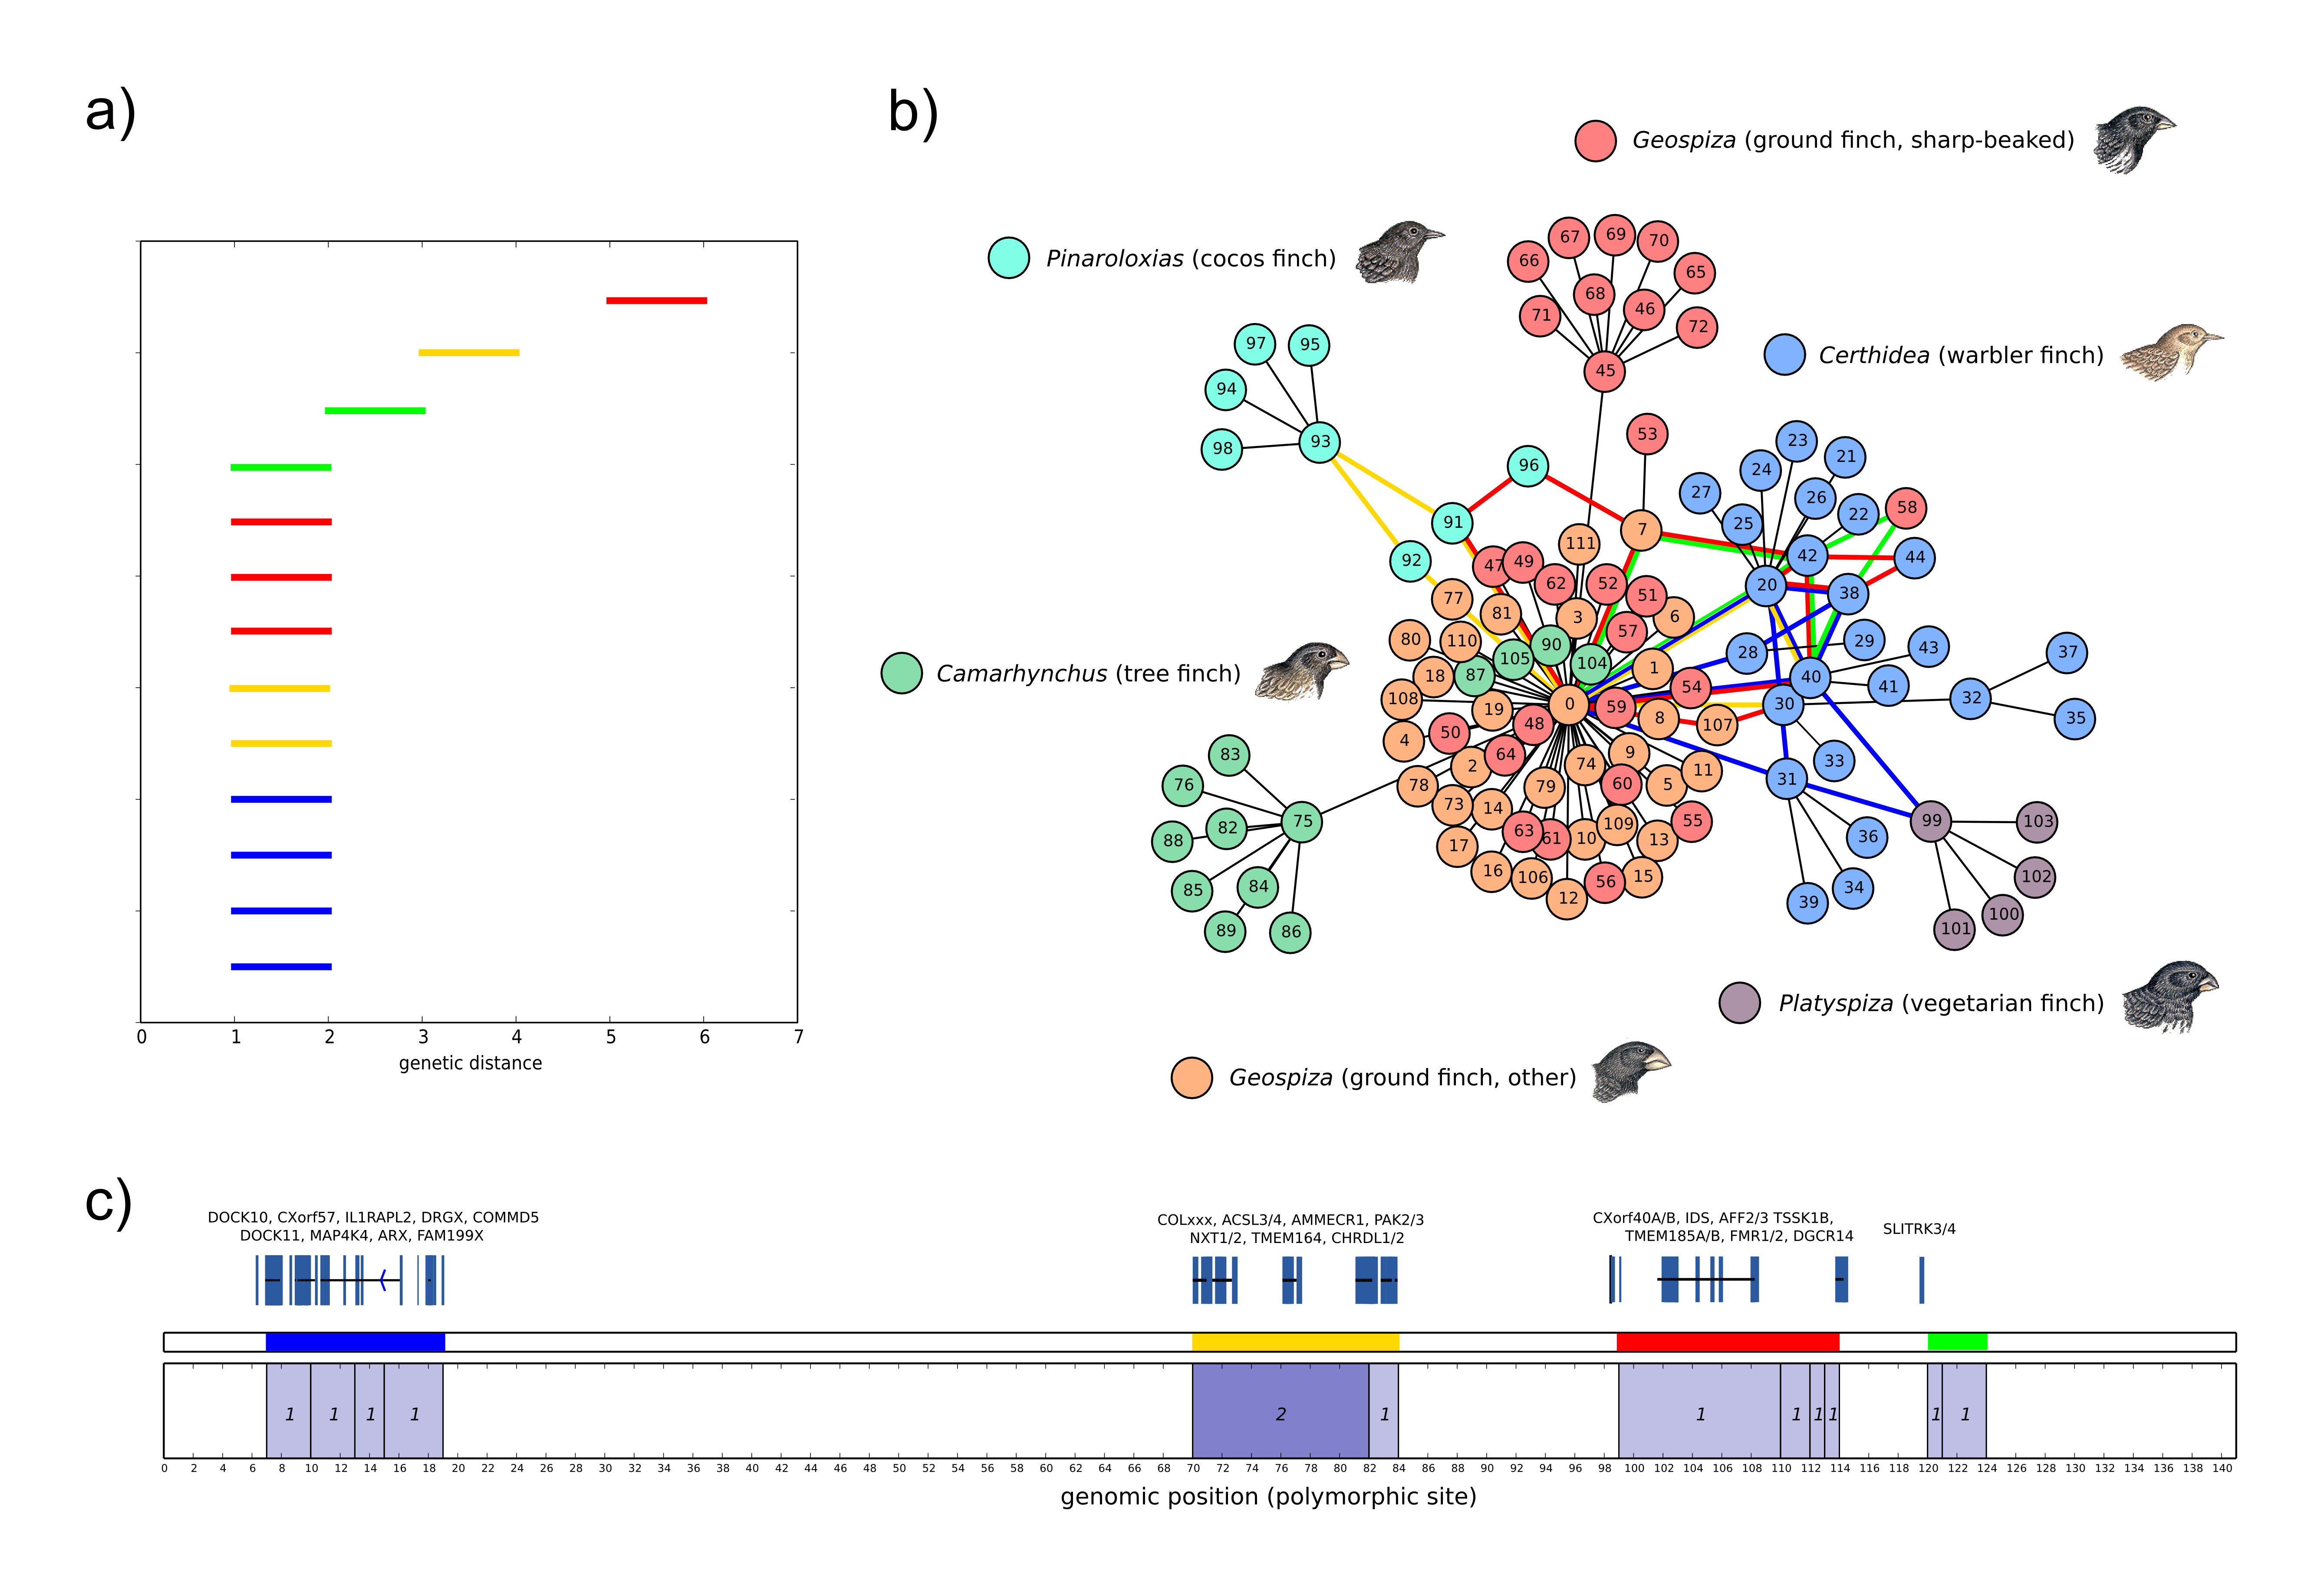
\includegraphics[width=16cm, angle=0]{finches.png}
\caption{Extended first-homology barcode and reconstructed tARG of a sample of 112 Darwin's finches, obtained with \texttt{TARGet} (the source FASTA file, \texttt{Darwing\_Finches.fa}, is included in the distribution). The extended first-homology barcode is shown in a), based on 140 homozygous SNPs present in a 9 megabase scaffold. In total, 13 recombination/gene flow events are captured in the extended barcode, having different genetic scales. Bars are coloured according to the position of the corresponding recombination breakpoint in the genome, as depicted in The number of recombination events detected at each genomic interval, as well as some of the orthologous genes present at regions where recombination events are detected, are indicated in c). The reconstructed tARG is presented in b). Recombination loops in the reconstructed tARG are outlined using the same code of colors. Leaf nodes that do not participate in any recombination event are also included in the graph, using a nearest neighbour algorithm based on genetic distance. Edge lengths are arbitrary. Figure taken from \cite{target}.
\label{fig7}}
\end{figure} 

\begin{thebibliography}{99}

\bibitem{ph} Edelsbrunner, H., Letscher, D. and Zomorodian, A. (2002), \emph{Topological persistence and simplification}. Discrete and Computational Geometry {\bf 69}, pp. 511-533.

\bibitem{ph2} Zomorodian, A. and Carlsson, G. (2005), \emph{Computing persistent homology}. Discrete and Computational Geometry {\bf 33}, pp. 247-274.

\bibitem{mg} Myers, S.R. and Griffiths, R.C. (2003), \emph{Bounds on the minimum number of recombination events in a sample history}. Genetics {\bf 163}, pp. 375-394.

\bibitem{target} Camara, P.G., Levine A.J. and Rabadan R. (2015), \emph{Inference of ancestral recombination graphs through topological data analysis}. In preparation.

\bibitem{hk} Hudson, R.R. and Kaplan, N.L. (1985), \emph{Statistical Properties of the Number of Recombination Events in the History of a Sample of DNA Sequences}. Genetics {\bf 111}, pp. 147-164.

\end{thebibliography}

\end{document}
          
